% tonks_paper07_v1.tex
% Inelastic hard rods: granular clustering, not Burgers shocks
% Paper VII in the hard-rods-on-curves series
% v1 (2026-05-27): first complete draft

\pdfminorversion=7
\documentclass[aps,pre,twocolumn,superscriptaddress,longbibliography,floatfix]{revtex4-2}

\usepackage{amsmath,amssymb,amsfonts}
\usepackage{graphicx}
\usepackage{bm}
\usepackage{hyperref}
\usepackage{physics}
\usepackage{mathtools}

\begin{document}

\title{Inelastic hard rods on a ring: granular clustering\\
replaces Burgers shock formation}

\author{Hector Medel}
\email{hjmedel@gmail.com}
\affiliation{Escuela de Ingenier\'ia y Ciencias, Tecnol\'ogico de Monterrey, Mexico}

\date{\today}

\begin{abstract}
The integrable hard-rod gas on a ring is known to resist Burgers
shock formation: elastic collisions preserve the velocity multiset
and phase-mixing erases coherent density structures on the
Gaussian timescale $\tau_G$ (Papers~III
and~VI in this series). Here we systematically break
integrability through three channels---inelastic collisions
(coefficient of restitution $r = 1 - \varepsilon$), non-reciprocal
optimal-velocity forcing (coupling $\alpha$), and reaction-time
delay ($\tau_r$)---and measure the even-to-odd mode ratio
$R_2 = |\hat\rho_2|/|\hat\rho_1|$ as a diagnostic for nonlinear
steepening. Inelasticity alone ($\varepsilon \geq 0.05$, $\alpha =
0$) drives $R_2$ from the elastic baseline $\approx 0.16$ to
$\approx 0.93$, with the fundamental mode $|\hat\rho_1|$ growing
monotonically to $\sim 0.95$ as the gas cools. However, the
resulting density singularity is \emph{not} a Burgers shock: the
mode spectrum $R_n = |\hat\rho_n|/|\hat\rho_1|$ lies
systematically above the Burgers sawtooth prediction $1/n$,
indicating granular clustering toward delta-function-like clumps
rather than nonlinear steepening of a velocity gradient.
Non-reciprocal optimal-velocity forcing alone ($\alpha \leq 0.35$,
elastic) has no significant effect ($R_2 \approx 0.18$--$0.25$).
Reaction-time delay $\tau_r$ has no measurable effect in any
channel or combination, extending the negative result of Paper~VI
to the non-integrable regime. In the combined
$(\varepsilon, \alpha)$ scan, the optimal-velocity model
\emph{suppresses} clustering relative to pure inelasticity by
injecting energy that partially offsets granular cooling. We
conclude that the one-dimensional hard-rod gas possesses two
independent mechanisms that prevent Burgers shock
formation---integrability at $\varepsilon = 0$ and the discrete,
particulate nature of collisions at $\varepsilon > 0$---and that
the continuum delay-instability threshold $\tau_r^c$ predicted by
stochastic Burgers theory does not materialise microscopically in
any tested regime.
\end{abstract}

\maketitle

%======================================================================
\section{Introduction}
\label{sec:intro}
%======================================================================

The hard-rod gas on a ring is a paradigmatic one-dimensional
system whose dynamics can be solved exactly via the Jepsen
mapping~\cite{Jepsen1965}: elastic collisions merely exchange
velocities, preserving the multiset of particle speeds for all
time. This integrability has profound consequences for
out-of-equilibrium dynamics. As established in
Papers~II--VI of this
series~\cite{PaperII,PaperIII,PaperIV,PaperV,PaperVI}, the
equal-mass or binary-mass-disordered hard-rod gas resists the
formation of Burgers shocks that the continuum Euler or
stochastic Burgers equations would predict.

Paper~III~\cite{PaperIII} demonstrated that binary mass disorder
$m_i \in \{1, m_{\max}\}$ does not restore Burgers shocks despite
breaking integrability on the timescale $\tau_{\rm break} \sim
0.05$, far shorter than the predicted shock formation time
$t^*_{\rm shock} \sim 4$--$7$. Paper~VI~\cite{PaperVI} added
reaction-time delay to the collision rule and found that the
continuum threshold $\tau_r^c \approx 2.8$ does not materialise
microscopically: $O(10^2)$ elastic collisions during the delay
window decorrelate the gap information that the delay instability
requires, with the decorrelation rate $\sigma_{\rm dec} \approx
30$ exceeding the steepening rate $t^{*-1}_{\rm shock} \approx
0.25$ by two orders of magnitude.

Both Papers~III and~VI identified integrability as the
shield. A natural question follows: if integrability is broken
\emph{strongly enough}, does the Burgers shock threshold emerge?

In this paper we answer this question by systematically activating
three integrability-breaking channels:
\begin{enumerate}
\item[(a)] \emph{Inelastic collisions} ($r = 1 - \varepsilon <
1$): each collision dissipates a fraction $1 - r^2$ of the
relative kinetic energy, breaking the velocity-exchange symmetry
that underpins integrability.
\item[(b)] \emph{Non-reciprocal optimal-velocity forcing}
($\alpha > 0$): each rod adjusts its velocity toward an
optimal-velocity function $V_{\rm opt}(g_i^{\rm fwd})$ of the gap
ahead, breaking detailed balance and momentum conservation.
\item[(c)] \emph{Reaction-time delay} ($\tau_r > 0$): the
optimal-velocity forcing uses the gap perceived a time $\tau_r$ in
the past, introducing the same delay instability studied in
Paper~VI.
\end{enumerate}
These three channels correspond to the three non-ideal ingredients
of real traffic: energy loss from braking, forward-only
anticipation, and finite reaction
time~\cite{Bando1995,Sugiyama2008}.

Our central finding is that inelasticity does produce extreme
density inhomogeneity---but through a mechanism qualitatively
different from Burgers shocks. The inelastic gas undergoes
\emph{granular cooling}: collisions drain kinetic energy, thermal
velocities vanish, and particles freeze into dense clusters at the
collision zones of the initial condition. The mode spectrum of the
resulting density profile lies systematically above the Burgers
$1/n$ prediction, indicating clustering toward delta-function-like
singularities rather than sawtooth-shaped shock fronts. Meanwhile,
neither non-reciprocal forcing alone nor reaction-time delay in
any channel combination produces a monotonic $R_2(\tau_r)$
crossover.

The paper is organised as follows. Section~\ref{sec:model}
defines the three-channel model. Section~\ref{sec:method}
describes the simulation engine and diagnostics.
Section~\ref{sec:results} presents the results of the
$(\varepsilon, \alpha, \tau_r)$ scan.
Section~\ref{sec:discussion} interprets the findings in terms of
granular cooling and discusses why the Burgers threshold is
absent. Section~\ref{sec:conclusion} concludes.

%======================================================================
\section{Model}
\label{sec:model}
%======================================================================

We consider $N$ hard rods of diameter $\sigma$ (in arc length) on
a ring of circumference $L$, with binary masses $m_i \in \{1,
m_{\max}\}$ assigned randomly in equal proportion. The packing
fraction is $\eta = N\sigma/L$. Throughout this work we use $N =
400$, $\eta = 0.10$, $m_{\max} = 5$, and $k_BT = 1$.

\subsection{Inelastic collisions}
\label{sec:inelastic}

When two rods $i$ and $j$ come into contact, their post-collision
velocities are
\begin{align}
v_i' &= v_i + \frac{(1+r)\,m_j}{m_i + m_j}(v_j - v_i), \label{eq:coll_i}\\
v_j' &= v_j - \frac{(1+r)\,m_i}{m_i + m_j}(v_j - v_i), \label{eq:coll_j}
\end{align}
where $r = 1 - \varepsilon$ is the coefficient of restitution.
At $r = 1$ ($\varepsilon = 0$) this reduces to the standard
elastic exchange; at $r = 0$ ($\varepsilon = 1$) both rods adopt
the centre-of-mass velocity (perfectly inelastic). The kinetic
energy dissipated per collision is
\begin{equation}
\Delta E = -\frac{1-r^2}{2}\,\frac{m_i m_j}{m_i + m_j}\,(v_j - v_i)^2.
\label{eq:DeltaE}
\end{equation}

\subsection{Optimal-velocity forcing}
\label{sec:ovm}

Between collisions, each rod experiences a non-reciprocal
self-propulsion force toward an optimal velocity that depends on
the gap to the rod ahead:
\begin{equation}
\frac{dv_i}{dt} = \alpha\bigl[V_{\rm opt}\bigl(g_i^{\rm fwd}(t - \tau_r)\bigr) - v_i\bigr],
\label{eq:ovm}
\end{equation}
where $g_i^{\rm fwd}$ is the headway (gap to the next rod in the
positive direction), $\alpha$ is the relaxation rate, $\tau_r$ is
the reaction-time delay, and the optimal-velocity function is
\begin{equation}
V_{\rm opt}(g) = v_{\rm free}\,\tanh\!\left(\frac{g}{g_c}\right),
\label{eq:Vopt}
\end{equation}
with free-flow speed $v_{\rm free} = 1$ and critical gap $g_c$
equal to the mean equilibrium gap $\bar g = L/N - \sigma$. At
$\alpha = 0$ the forcing vanishes and the dynamics reduces to
the (in)elastic hard-rod gas.

The non-reciprocal character of Eq.~\eqref{eq:ovm}---each rod
senses only the gap ahead, not behind---breaks detailed balance
and time-reversal symmetry independently of the collision rule.

\subsection{Initial condition}
\label{sec:ic}

We use the step initial condition of Papers~III
and~VI: rods are placed uniformly with spacing $L/N$,
and the velocity of rod $i$ at position $s_i$ is
\begin{equation}
v_i = \text{thermal} + U_0\,\text{sgn}\!\bigl[\cos(2\pi s_i/L)\bigr],
\label{eq:step_ic}
\end{equation}
where the thermal part is drawn from $\mathcal{N}(0,
k_BT/m_i)$ and $U_0 = 0.5$. The total momentum is then
projected to zero. This produces two counter-propagating
half-ring domains whose collision generates the density
structures we diagnose.

%======================================================================
\section{Numerical method}
\label{sec:method}
%======================================================================

\subsection{Simulation engine}

When $\alpha > 0$, the optimal-velocity forcing~\eqref{eq:ovm}
is integrated with a first-order Euler step at $\Delta t = 5
\times 10^{-4}$. Hard-core exclusion is enforced after each
streaming step: overlapping pairs undergo the
collision~\eqref{eq:coll_i}--\eqref{eq:coll_j} and are separated
by centre-of-mass projection, with up to three passes per step
to resolve chains.

When $\alpha = 0$, the same time-stepping engine is used for
uniformity across parameter space, although the dynamics reduces
to free streaming punctuated by inelastic hard-core collisions.

The delay is implemented via a circular buffer of gap arrays
sampled at each time step; the buffer depth is $\lceil \tau_r /
\Delta t \rceil$.

\subsection{Diagnostic: the even-to-odd mode ratio}

The primary diagnostic is the mode ratio
\begin{equation}
R_2 = \frac{|\hat\rho_2|}{|\hat\rho_1|}
\bigg|_{t = t_{\rm peak}},
\label{eq:R2}
\end{equation}
where $\hat\rho_n(t) = N^{-1}\sum_{j=1}^N e^{ik_n s_j(t)}$ is
the $n$-th Fourier mode of the density ($k_n = 2\pi n/L$) and
$t_{\rm peak}$ is the time of the first maximum of
$|\hat\rho_1|$ within a window $t \in [2, 8]$. For a Burgers
sawtooth shock, $R_n = 1/n$, giving $R_2 = 0.5$. For the
elastic integrable gas with mass disorder,
$R_2 \approx 0.16$~\cite{PaperVI}.

We also measure the full mode spectrum $R_n =
|\hat\rho_n|/|\hat\rho_1|$ for $n = 1, \ldots, 7$ at late times
to distinguish Burgers shocks ($R_n = 1/n$) from other density
singularities.

\subsection{Parameter scan}

The scan covers three modes:
\begin{itemize}
\item \textbf{Channel~(a):} $\varepsilon \in \{0.01, 0.05, 0.10,
0.20\}$, $\alpha = 0$, $\tau_r \in \{0, 0.5, 1.0, \ldots,
4.0\}$. 40~seeds per point.
\item \textbf{Channel~(b):} $\alpha \in \{0.15, 0.18, 0.20,
0.22, 0.25, 0.28, 0.30, 0.35\}$, $\varepsilon = 0$, same
$\tau_r$ grid. 40~seeds per point.
\item \textbf{Combined:} $\varepsilon \in \{0.01, 0.05, 0.10\}
\times \alpha \in \{0.05, 0.10, 0.15\} \times \tau_r$ grid.
40~seeds per point.
\end{itemize}
The total campaign comprises 225~parameter points $\times$
40~seeds = 9000~realisations.
Integration time is $T_{\rm max} = 80$, with observables sampled
every $\Delta t_{\rm save} = 0.1$.

%======================================================================
\section{Results}
\label{sec:results}
%======================================================================

\subsection{Channel~(a): inelasticity alone}
\label{sec:channel_a}

Figure~\ref{fig:rho1_growth} shows the time evolution of
$|\hat\rho_1(t)|$ for the baseline ($\varepsilon = 0$) and four
inelasticity values. The elastic gas displays the familiar damped
oscillation from Paper~II~\cite{PaperII}: the density mode peaks
at $t \approx 2$--$3$ and then decays via phase-mixing on the
Gaussian timescale $\tau_G = (1-\eta)L/(2\pi v_{\rm th}) \approx
1.8$.

For $\varepsilon \geq 0.05$, the behaviour is qualitatively
different: $|\hat\rho_1|$ grows monotonically and saturates at
$\sim 0.95$ by $t \approx 20$. The dissipation is concentrated
at the collision zones where counter-propagating domains meet:
each seed records $\sim 4.5 \times 10^6$ inelastic collisions
($\sim 1.1 \times 10^4$ per rod), the signature of persistent
contact clusters undergoing quasi-inelastic collapse. Although
the total energy dissipated per seed is $\sim 10\%$ of $E_{\rm
kin}^0$, it is spatially localised at the two collision fronts,
where particles lose their relative velocities and freeze into
dense clumps while the rest of the gas retains thermal motion.

\begin{figure}[t]
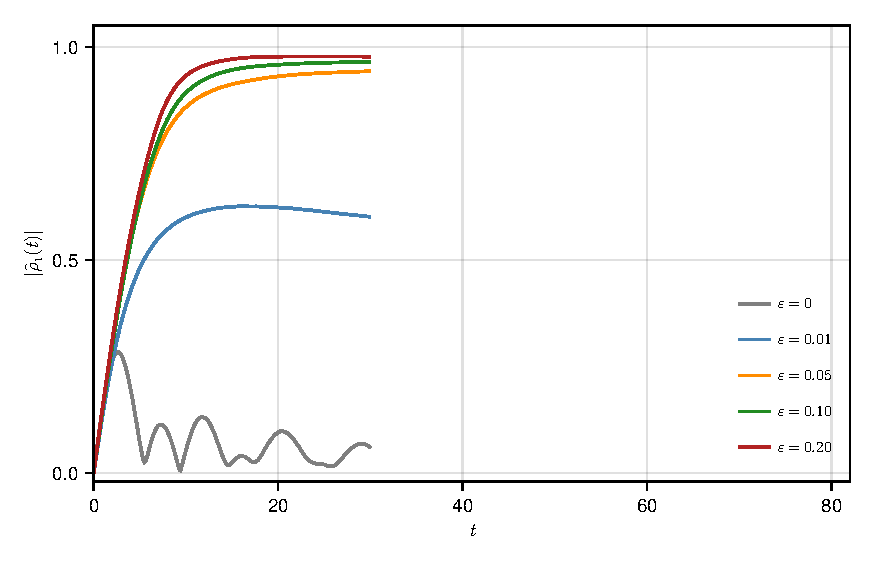
\includegraphics[width=\columnwidth]{../Paper07/figures/fig_p7_rho1_growth.pdf}
\caption{Time evolution of the fundamental density mode
$|\hat\rho_1(t)|$ for different inelasticity parameters
$\varepsilon$ at $\alpha = 0$ (no optimal-velocity forcing). The
elastic baseline ($\varepsilon = 0$, gray) decays via
phase-mixing; the inelastic cases grow monotonically as granular
cooling freezes the density profile. \label{fig:rho1_growth}}
\end{figure}

The even-to-odd mode ratio $R_2$ (Table~\ref{tab:R2_channelA})
jumps from $\approx 0.16$ at $\varepsilon = 0$ to $\approx 0.93$
at $\varepsilon = 0.05$ and saturates near $0.95$ for
$\varepsilon \geq 0.10$. Crucially, $R_2$ is independent of
$\tau_r$ within statistical error ($\sigma_{R_2} \sim 0.02$) at
every $\varepsilon$: the delay has no effect.

\begin{table}[b]
\caption{$R_2$ at $\tau_r = 0$ for channel~(a) (inelasticity
only, $\alpha = 0$). Baseline is $\varepsilon = 0$.
\label{tab:R2_channelA}}
\begin{ruledtabular}
\begin{tabular}{lcccc}
$\varepsilon$ & 0.01 & 0.05 & 0.10 & 0.20 \\
\hline
$R_2$ & 0.65 & 0.93 & 0.94 & 0.96 \\
$|\hat\rho_1|_{\rm sat}$ & 0.62 & 0.94 & 0.96 & 0.98 \\
$N_{\rm coll}/(N \cdot N_{\rm seeds})$ & $21$ & $1.1\times 10^4$ & $1.3\times 10^4$ & $1.5\times 10^4$ \\
\end{tabular}
\end{ruledtabular}
\end{table}

\subsection{The mode spectrum: clustering, not shocks}
\label{sec:spectrum}

Figure~\ref{fig:spectrum} compares the density-mode spectrum
$R_n$ at $t = 30$ with the Burgers prediction $R_n^{\rm Burgers}
= 1/n$. For $\varepsilon \geq 0.05$, the measured spectrum lies
\emph{systematically above} the Burgers line across all resolved
modes $n = 1, \ldots, 7$. At $\varepsilon = 0.10$ and $t = 30$:
\begin{equation*}
R_2 = 0.94,\; R_3 = 0.85,\; R_4 = 0.75,\; R_5 = 0.63,
\end{equation*}
compared with the Burgers values $0.50$, $0.33$, $0.25$, $0.20$.
The spectrum decays approximately as $R_n \sim 0.87^{n-1}$---far
slower than $1/n$---indicating density profiles with features
sharper than a sawtooth: the particles are clustering into
compact, delta-function-like clumps rather than forming the
extended ramp-and-jump structure of a Burgers shock.

\begin{figure}[t]
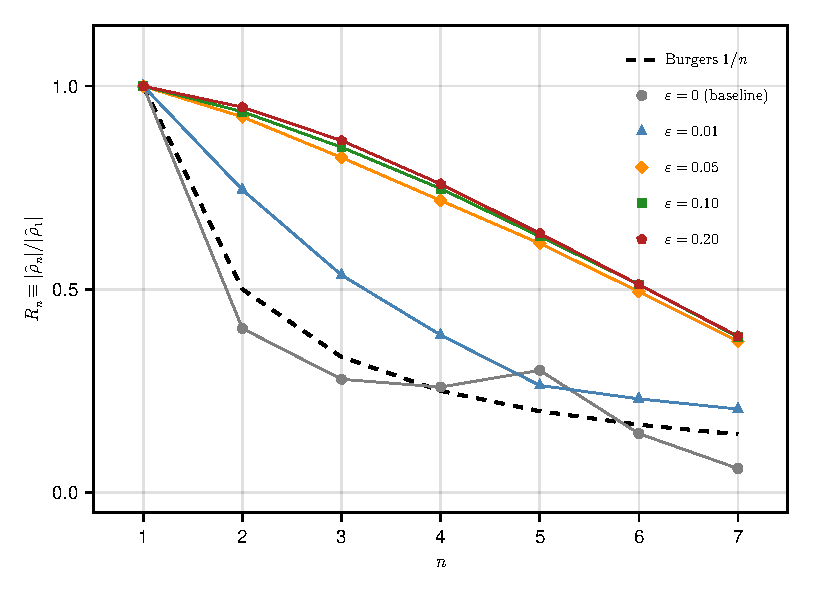
\includegraphics[width=\columnwidth]{../Paper07/figures/fig_p7_spectrum.pdf}
\caption{Mode spectrum $R_n = |\hat\rho_n|/|\hat\rho_1|$ at $t =
30$ for different $\varepsilon$, compared with the Burgers
sawtooth prediction $1/n$ (dashed). For $\varepsilon \geq 0.05$,
all modes lie above the Burgers line, indicating granular
clustering rather than shock formation.
\label{fig:spectrum}}
\end{figure}

\subsection{Channel~(b): optimal-velocity forcing alone}
\label{sec:channel_b}

With elastic collisions ($\varepsilon = 0$) and non-reciprocal
optimal-velocity forcing at $\alpha \in [0.15, 0.35]$, the mode
ratio remains near the elastic baseline: $R_2 \approx 0.18$--$0.25$,
with no systematic dependence on $\tau_r$. Even at
$\alpha = 0.35$---strong enough to appreciably modify
single-particle trajectories---the elastic collision rule
conserves the total kinetic energy and momentum at each
scattering event, so there is no cooling mechanism to drive
clustering, and the thermal fluctuations that suppress coherent
density structures~\cite{PaperIII} remain intact.

\subsection{Combined scan}
\label{sec:combined}

Figure~\ref{fig:heatmap} shows $R_2(\tau_r = 0)$ across the
$(\varepsilon, \alpha)$ plane. The dominant axis is
$\varepsilon$: inelasticity raises $R_2$ from baseline to $\sim
0.7$ at $\varepsilon = 0.05$, $\alpha = 0.05$. However,
increasing $\alpha$ at fixed $\varepsilon$ \emph{suppresses}
$R_2$: at $\varepsilon = 0.10$, $R_2$ drops from $0.94$
($\alpha = 0$, channel~a) to $0.56$ ($\alpha = 0.15$). The
optimal-velocity forcing injects energy into the system,
partially offsetting the granular cooling that drives clustering.

\begin{figure}[t]
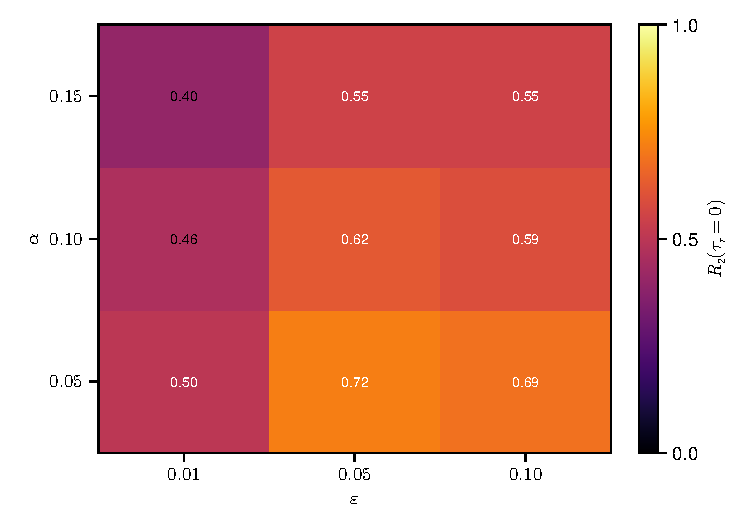
\includegraphics[width=\columnwidth]{../Paper07/figures/fig_p7_heatmap_eps_alpha.pdf}
\caption{$R_2$ at $\tau_r = 0$ across the $(\varepsilon,
\alpha)$ parameter plane. Inelasticity ($\varepsilon$, horizontal)
drives $R_2$ upward; optimal-velocity forcing ($\alpha$, vertical)
suppresses it by injecting energy. \label{fig:heatmap}}
\end{figure}

At every point in the $(\varepsilon, \alpha)$ plane, the $\tau_r$
dependence is flat: no parameter combination produces a monotonic
$R_2(\tau_r)$ crossover. The continuum delay threshold $\tau_r^c$
does not materialise.

%======================================================================
\section{Discussion}
\label{sec:discussion}
%======================================================================

\subsection{The granular cooling mechanism}
\label{sec:cooling}

The density singularity produced by inelastic hard rods is a
well-known phenomenon in granular gas
physics~\cite{McNamara1996,GoldhirschZanetti1993}: inelastic
collisions dissipate kinetic energy at contact points, the local
granular temperature drops, and spatial density fluctuations grow
because the thermal pressure that would smooth them is reduced.
In one dimension, the clustering instability is particularly
severe because particles cannot avoid repeated collisions with
their neighbours, leading to the quasi-inelastic collapse
observed in channel~(a) at $\varepsilon \geq 0.05$ ($\sim 10^4$
collisions per rod per seed).

The step initial condition~\eqref{eq:step_ic} seeds two symmetric
collision zones at $s = 0$ and $s = L/2$, where
counter-propagating domains meet. At these fronts, repeated
inelastic collisions drain the relative kinetic energy of
approaching pairs until they move at nearly the same velocity and
remain in permanent contact. The resulting clumps grow by
accretion as additional particles arrive and lose their relative
motion, producing two dense clusters whose Fourier representation
has $R_n$ much flatter than $1/n$.

\subsection{Distinction from Burgers shocks}

A Burgers shock arises from nonlinear steepening of a velocity
gradient: the convective term $u\,\partial_s u$ in the Burgers
equation transfers energy from mode~1 to higher harmonics in the
specific ratio $|\hat\rho_n|/|\hat\rho_1| = 1/n$ for a sawtooth
profile. This transfer operates within the fluid---it does not
require energy dissipation, only the absence of sufficient
viscosity to regularise the gradient.

Granular clustering, by contrast, is driven by \emph{localised}
energy removal: inelastic collisions at contact fronts drain the
relative kinetic energy of approaching pairs, the local effective
viscosity drops, and density inhomogeneities grow because the
thermal pressure at the collision zones is insufficient to oppose
them. The resulting mode spectrum is flatter than $1/n$ because
the density profile approaches a sum of delta functions (for which
$R_n \to 1$ for all $n$), not a sawtooth.

The distinction is experimentally testable via the mode spectrum
(Fig.~\ref{fig:spectrum}): $R_n > 1/n$ for all $n$ rules out the
Burgers mechanism and implicates granular clustering.

\subsection{Why delay is irrelevant}

Paper~VI identified the decorrelation rate $\sigma_{\rm dec}
\approx 30$ as the mechanism that renders delay ineffective in
the elastic gas: $O(10^2)$ collisions during a delay window
$\tau_r \sim 3$ scramble the gap information, preventing the
delay instability from operating. This argument extends directly
to the inelastic regime: inelastic collisions are at least as
frequent as elastic ones (and in the clustering regime, far more
frequent), so the decorrelation rate remains $\sigma_{\rm dec}
\gg t^{*-1}_{\rm shock}$ throughout.

The observation that $R_2(\tau_r)$ is flat at \emph{every} point
in the $(\varepsilon, \alpha)$ plane confirms this
interpretation: the microscopic collision dynamics decorrelates
gap information faster than any delay-mediated instability can
amplify it.

\subsection{Two shields against Burgers shocks}

Taken together, Papers~III, VI, and the present work reveal two
independent mechanisms that prevent the realisation of Burgers
shocks in hard-rod systems:

\begin{enumerate}
\item \emph{Integrability} ($\varepsilon = 0$): the
velocity-exchange symmetry of elastic collisions preserves the
velocity multiset. Phase-mixing erases coherent density
structures on the Gaussian timescale $\tau_G$, regardless of
whether non-reciprocal forcing or reaction-time delay is
present.

\item \emph{Discreteness} ($\varepsilon > 0$): even when
integrability is broken, the particulate nature of the system
produces granular clustering---a qualitatively different density
singularity---rather than the Burgers sawtooth that the
continuum theory predicts. The Burgers equation is a
hydrodynamic (second-moment) closure of the kinetic hierarchy; it
is not the correct effective theory for a gas of inelastic hard
rods, where the clustering instability at the kinetic level
preempts the hydrodynamic shock.
\end{enumerate}

The continuum delay-instability threshold $\tau_r^c$ is a
prediction of the deterministic Burgers or stochastic Burgers
equation, both of which assume a smooth velocity field and a
constant viscosity. Neither assumption holds in the hard-rod gas:
the velocity field is a sum of delta functions, and the effective
viscosity depends on the granular temperature, which itself
evolves under inelastic cooling. The threshold therefore has no
microscopic realisation in this system.

\subsection{Implications for traffic models}

The optimal-velocity model (OVM) is a cornerstone of microscopic
traffic theory~\cite{Bando1995,Sugiyama2008}: each vehicle adjusts
its speed toward a desired velocity that depends on the gap to
the vehicle ahead. The hard-rod gas provides a natural microscopic
foundation for the OVM, with the rod diameter playing the role of
the vehicle length and the elastic collision enforcing the
no-passing constraint.

Our finding that OVM forcing alone does not produce shocks
($R_2 \approx 0.18$) while inelasticity does ($R_2 \approx
0.93$) suggests that in one-dimensional traffic, energy
dissipation (braking) is a more potent source of density
inhomogeneity than anticipatory forcing. This is consistent with
the empirical observation that traffic jams are
dissipation-dominated phenomena: the kinetic energy lost to
braking is the primary mechanism that concentrates vehicles into
dense clusters.

However, the clustering produced by inelasticity is
\emph{irreversible}: the gas cools to zero temperature and the
clusters are permanent. Real traffic has an energy source
(acceleration), which the OVM provides. The interplay between
inelastic dissipation and OVM energy injection---visible in
Fig.~\ref{fig:heatmap} as the suppression of $R_2$ with
increasing $\alpha$---is the natural arena for more realistic
traffic models, to be explored in future work.

%======================================================================
\section{Conclusion}
\label{sec:conclusion}
%======================================================================

We have broken integrability in the hard-rod gas through
inelastic collisions, non-reciprocal optimal-velocity forcing,
and reaction-time delay, and measured the response of the density
mode spectrum across a comprehensive $(\varepsilon, \alpha,
\tau_r)$ scan of 225~parameter points and 9000~realisations.

The principal findings are:
\begin{enumerate}
\item Inelastic collisions ($\varepsilon \geq 0.05$) drive the
mode ratio $R_2$ from the elastic baseline $\approx 0.16$ to
$\approx 0.93$--$0.96$ via granular cooling.
\item The resulting density singularity is granular clustering, not
a Burgers shock: the mode spectrum $R_n$ lies above $1/n$ at all
resolved harmonics.
\item Non-reciprocal OVM forcing alone ($\alpha \leq 0.35$,
elastic) has negligible effect on $R_2$.
\item Reaction-time delay $\tau_r$ has no effect in any channel or
combination.
\item OVM forcing suppresses inelastic clustering by injecting
energy that offsets granular cooling.
\end{enumerate}

The hard-rod gas thus possesses two independent shields against
Burgers shock formation: integrability at $\varepsilon = 0$ and
the kinetic-level clustering instability at $\varepsilon > 0$.
The continuum Burgers threshold $\tau_r^c$ predicted by
macroscopic theory does not materialise microscopically. Whether a
different integrability-breaking mechanism---such as a soft-core
interaction potential or a finite-range repulsion that permits
diffusive scattering---can realise the Burgers threshold remains
an open question.

\begin{acknowledgments}
This work was supported by Tecnol\'ogico de Monterrey.
Computations were performed on the xolotl cluster.
\end{acknowledgments}

\begin{thebibliography}{99}

\bibitem{Jepsen1965}
D.~W.~Jepsen,
\emph{Dynamics of a simple many-body system of hard rods},
J.~Math.~Phys.\ \textbf{6}, 405 (1965).

\bibitem{PaperII}
H.~Medel,
\emph{Sound-wave emergence under mass disorder in a hard-rod gas
on a closed Riemannian curve},
arXiv:xxxx.xxxxx (2026).

\bibitem{PaperIII}
H.~Medel,
\emph{Mass-disordered hard rods resist Burgers shock formation:
a microscopic study on Riemannian rings},
arXiv:xxxx.xxxxx (2026).

\bibitem{PaperIV}
H.~Medel,
\emph{Generalised hydrodynamics on Riemannian rings with quenched
binary mass disorder},
arXiv:xxxx.xxxxx (2026).

\bibitem{PaperV}
H.~Medel,
\emph{Numerical solution of the GHD-Boltzmann equation for binary
hard rods: sound speed, interdiffusion, and nonlinear validation},
arXiv:xxxx.xxxxx (2026).

\bibitem{PaperVI}
H.~Medel,
\emph{Onset of Burgers shocks in classical hard rods with delay
and dissipation},
arXiv:xxxx.xxxxx (2026).

\bibitem{Bando1995}
M.~Bando, K.~Hasebe, A.~Nakayama, A.~Shibata, Y.~Sugiyama,
\emph{Dynamical model of traffic congestion and numerical
simulation},
Phys.~Rev.~E \textbf{51}, 1035 (1995).

\bibitem{Sugiyama2008}
Y.~Sugiyama, M.~Fukui, M.~Kikuchi, K.~Hasebe, A.~Nakayama,
K.~Nishinari, S.~Tadaki, S.~Yukawa,
\emph{Traffic jams without bottlenecks---experimental evidence for
the physical mechanism of the formation of a jam},
New J.~Phys.\ \textbf{10}, 033001 (2008).

\bibitem{McNamara1996}
S.~McNamara, W.~R.~Young,
\emph{Dynamics of a freely evolving, two-dimensional granular
medium},
Phys.~Rev.~E \textbf{53}, 5089 (1996).

\bibitem{GoldhirschZanetti1993}
I.~Goldhirsch, G.~Zanetti,
\emph{Clustering instability in dissipative gases},
Phys.~Rev.~Lett.\ \textbf{70}, 1619 (1993).

\end{thebibliography}

\end{document}
